\chapter{Revisão da Literatura}
\label{cap:descr}

%% - - - - - - - - - - - - - - - - - - - - - - - - - - - - - - - - - - -
\section{O Teste palográfico}
\label{sec:testep}
O teste dos palos tem como objetivo fazer uma avaliação da personalidade do indivíduo. É muito utilizado em empresas no recrutamento e seleção, para conseguir selecionar os melhores profissionais do mercado e garantir compatibilidade entre os profissionais selecionados com as exigências da vaga. 

O teste palográfico foi desenvolvido na Espanha e trazido para o Brasil por Agostinho Minicucci na década de 1970. O instrumento é considerado um teste expressivo de personalidade,  que tem como base teórica, questões relativas ao comportamento expressivo e técnicas gráficas para avaliação da personalidade.\cite{ibapnet2012} Personalidade é o conjunto de características  físicas, genéticas e sociais que faz de um individuo diferente e único. \cite{dicio2018}

O teste palográfico depende da forma como a pessoa traça riscos numa folha, o psicólogo irá fazer uma análise da sua personalidade, verificando dados de ritmo e qualidade de trabalho, fatigabilidade, inibição, elação, depressão, temperamento, inteligencia, etc. \cite{manualPsico2010}

\section{Aplicação e correção do Teste}
\label{sec:formateste}
Ao aplicar o teste o psicologo não se diz aos candidatos do que se trata, apenas diz que é um teste de resistência e velocidade.

É fornecida uma folha em branco sem linhas. Nessa folha vem de exemplo 3 palos no começo da folha e abaixo desses 3 palos tem mais 1 palo impresso, com altura de 7mm,  e espaçados de 2 em 2 mm que devem ser replicados por quem for fazer o teste. A pessoa deve fazer de lápis, riscos verticais o quanto puder e o mais perfeito possível, no tempo de 5 minutos. \cite{manualPsico2010}

Para cada minuto o psicologo dará o comando "sinal", então a pessoa deverá riscar um traço na horizontal, e continuar a fazer os traços na vertical. ex:
|||||||||||||||||||-|||||||||||||||||-|||||||||||||||||||-|||||||||||||||||||-|||||||||||||||||
Antes de começar há um treino inicial e só depois é iniciando o teste. \cite{manualPsico2010}

O teste é muito utilizado em RH para fazer contratações  e no Detran (para autorizar a carteira de habilitação). \cite{kenoby2017}

A avaliação do teste palográfico é abordada de maneira quantitativa e qualitativa\footnote{ Para mais informações sobre a parte qualitativa acesse o manual do psicotécnico p. 355: https://aderivaldo23.files.wordpress.com/2008/06/37527582-manual-do-psicotecnico-1.pdf.}, esse trabalho se restringe apenas a parte quantitativa.

\subsection{Folhas do teste}
\label{sec:folhasTeste}

Existem dois modelos de folhas para realização do teste, um grande (36,3 x27,4 cm) e outro reduzido (21,5 x 32,0 cm). Em geral o mais utilizado é o reduzido, devido a limitação do tamanho das carteiras dos examinadores. Neste trabalho os testes focaram no modelo reduzido.\cite{passetestepalografico2013}


\begin{figure}[H]
 \centering
 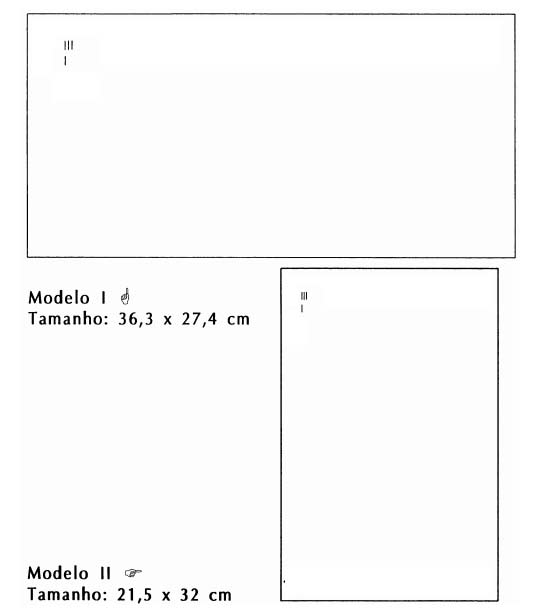
\includegraphics[width=0.76\textwidth]{./fig/palos/folhas}
 \caption{Modelos de folhas para aplicação do teste palográfico.}
  Fonte: \cite{passetestepalografico2013}.
 \label{fig:folhas}
\end{figure}


\subsection{Avaliação Quantitativa}
\label{sub:avaquali}

Nessa análise são considerados produtividade, rítmo, e rendimento.

\subsubsection{Produtividade}
\label{subsub:avaquali}

É a quantidade total de riscos, somando-se os 5 tempos.
Segundo \cite{marcosjaime2013}  a produtividade pode ser analisada de acordo com a quantidade de palos que a pessoa conseguiu fazer, compara-se com uma faixa de valores padrão de acordo com sua escolaridade, para fazer a classificação conforme pode se ver abaixo.

Candidatos (as) com escolaridade NÍVEL MÉDIO
\begin{itemize}
\item Menor ou igual 313: Inferior ou Lento - Indica uma produtividade muito abaixo da média.
\item De 314 a 423: Média Inferior ou Baixa - Índice demonstra um rendimento no trabalho abaixo da média.
\item De 424 a 693: Média - Indica possuir produtividade mediana no trabalho.
\item De 694 a 936: Média Superior ou Alta - Denota possuir produtividade acima da média.
\item  A partir de 937: Superior ou Muito Alta - Este índice revela produtividade acentuada no trabalho, indicando rendimento bastante acima da média.
\end{itemize}

Candidatos com escolaridade até NÍVEL SUPERIOR :

\begin{itemize}
\item Até 396: Inferior ou Lento - Indica uma produtividade muito abaixo da média.
\item De 397 a 546: Média Inferior ou Baixa - Este índice denota um rendimento no trabalho abaixo da média.
\item De 547 a 830: Média - Indica possuir produtividade mediana no trabalho.
\item De 831 a 1059: Média Superior ou Alta - Denota possuir produtividade acima da média.
\item A partir de 1060: Superior ou Muito Alta - Este índice revela produtividade acentuada no
trabalho, indicando rendimento bastante acima da média.
\end{itemize}

\subsubsection{Ritmo}
\label{subsub:ritmo}

Na avaliação do ritmo faz-se a soma da diferença na quantidade de palos entre cada um dos 5 tempos, proporcional ao total de palos na soma dos 5 tempos. Quanto mais baixo o nível de oscilação do ritmo, melhor. Isso pode também ser chamado de NOR - (Nível de Oscilação Rítmica. A fórmula é: NOR= (soma das diferenças)*100/(total de palos).\cite{marcosjaime2013} 

Ex: Palos 107/103/115/110/109 = 544 (total de palos)
Diferença: 4/12/5/1 = 22 (soma das diferenças)
(22x100)/544 = 4 (NOR)

De acordo com a o seu valor de NOR o avaliado pode ser classificado utilizando-se a faixa de valores para o NOR conforme abaixo. \cite{marcosjaime2013}

\begin{itemize}
\item NOR: 0,0 a 2,1: Muito Baixo - Indica rígida regularidade na execução das tarefas, capaz de manter uma produtividade constante.
\item NOR: 2,2 a 4,0: Baixo - Revela produtividade estável no trabalho, capaz de manter rendimento constante.
\item NOR: 4,1 a 8,7: Médio - Revela alguma instabilidade em sua produtividade, porém sendo capaz de executar satisfatoriamente tarefas repetitivas.
\item NOR: 8,8 a 13,2: Alto - Indicativo de oscilações na produtividade e rendimento irregular no trabalho.
\item NOR: a partir de 13,3: Muito Alto – Revela preocupante oscilação na produtividade demonstrando rendimento bastante irregular.
\end{itemize}

\subsubsection{Rendimento}
\label{subsub:rend}

A análise do rendimento é feita por um gráfico que da uma visão mais clara da relação entre a produtividade e o ritmo. Aqui é analisado a qualidade do rendimento no trabalho e a tendência à exaustão. No gráfico é analisado os tempos x quantidade de palos sendo os tempos no eixo das abcissas e a quantidade de palos no eixo das ordenadas. Para que a oscilação na produtividade seja melhor observada, deve-se sempre fazer o eixo vertical partindo do zero \cite{psicohood2018}.

Abaixo mostro como é feito a analise do gráfico de rendimento com alguns exemplos segundo os autores \cite{psicohood2018} e \cite{manualPsico2010}.

\textbf{Equilibrado} (NOR entre 4 e 6, com produção média): indica capacidade e distribuição do tônus muscular de forma organizada e sistemática. Revela realização de trabalho uniforme.

Ex.:

\begin{table*}[hp]
\caption{Rendimento equilibrado \cite{psicohood2018} }
\label{tab:equilibrado}

\centering
\begin{tabular}{|l|c|c|c|c|c|c|}
\hline   \multicolumn{1}{|l|}{Tempos}   & 1     & 2     & 3    &  4     & 5     & Total \\ 
\hline Nº de traços & 120 & 130 & 125 & 133 & 142 & 650 \\ 
\hline    \multicolumn{2}{|l|}{ Diferenças}& 10   & 5     & 8     & 9     & 32\\ 
\hline NOR = 4,9\\
\cline{1-11}
\end{tabular} 

\end{table*}

\begin{figure}[H]
 \centering
 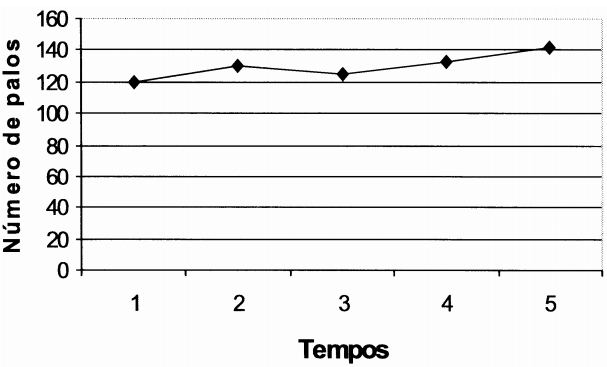
\includegraphics[width=0.76\textwidth]{./fig/grafico-rendimento/equilibrado}
 \caption{Rendimento equilibrado.}
  Fonte: \cite{psicohood2018}.
 \label{fig:folhas}
\end{figure}

\textbf{Rígido} (NOR entre 0 e 3, com produção média ou baixa): reflete pessoa obsessiva por detalhes e organização,
com rigidez da personalidade.

Ex.:
\begin{table*}[hp]
\caption{Rendimento rígido \cite{psicohood2018} }
\label{tab:rigido} 
\centering
\begin{tabular}{|l|c|c|c|c|c|c|}
\hline Tempos       & 1     & 2     & 3    &  4     & 5     & Total \\ 
\hline Nº de traços & 100 & 102 & 103 & 101 & 104 & 510 \\ 
\hline    \multicolumn{2}{|l|}{ Diferenças}& 2   & 1     & 2     & 3     & 8\\ 
\hline NOR = 1,6 \\ \cline{1-1}
\end{tabular} 

\end{table*}

\begin{figure}[H]
 \centering
 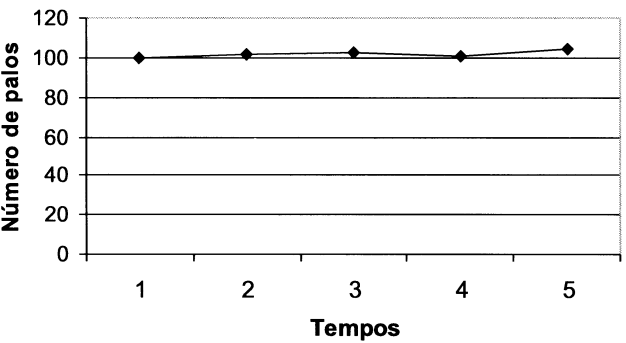
\includegraphics[width=0.76\textwidth]{./fig/grafico-rendimento/rigido}
 \caption{Rendimento rígido.}
  Fonte: \cite{psicohood2018}.
 \label{fig:folhas}
\end{figure}

\textbf{Ascendente ou crescente} (NOR acima de 6, com produção média): indica prudência diante de uma nova tarefa, mas aumenta a produção à medida que o indivíduo se sente mais seguro na situação. Também significa dinamismo e iniciativa.

Ex.:
\begin{table*}[hp]
\caption{Rendimento ascendente ou crescente \cite{psicohood2018} }
\label{tab:ascende} 
\centering
\begin{tabular}{|l|c|c|c|c|c|c|}
\hline Tempos       & 1     & 2     & 3    &  4     & 5     & Total \\ 
\hline Nº de traços & 110 & 125 & 135 & 140 & 155 & 665 \\ 
\hline    \multicolumn{2}{|l|}{ Diferenças}& 15   & 10     & 5     & 15    & 45\\ 
\hline NOR = 6,7\\  \cline{1-1}
\end{tabular} 

\end{table*}

\begin{figure}[H]
 \centering
 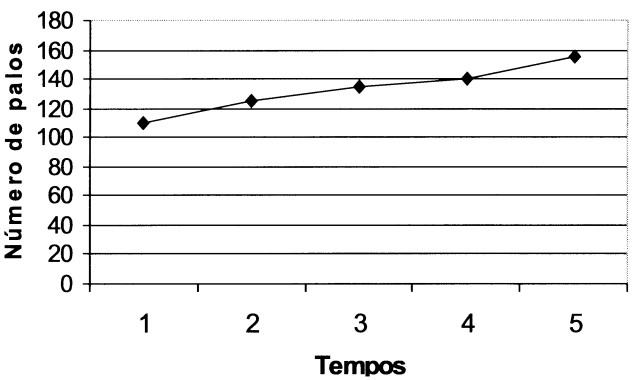
\includegraphics[width=0.76\textwidth]{./fig/grafico-rendimento/crescente}
 \caption{Rendimento ascendente ou crescente.}
  Fonte: \cite{psicohood2018}.
 \label{fig:ascende}
\end{figure}

\textbf{Descendente ou decrescente} (NOR acima de 6): é indicativo de cansaço, fadiga ou estresse, dificuldade de manter o tônus muscular, falta de ânimo e disposição. Pode refletir também tendência à depressão.

Ex.:

\begin{table*}[h]
\centering
\caption{Rendimento descendente ou decrescente \cite{psicohood2018} }

\label{tab:decrescente}


\begin{tabular}{|l|c|c|c|c|c|c|}
\hline Tempos       & 1     & 2     & 3    &  4     & 5     & Total \\ 
\hline Nº de traços & 180 & 175 & 150 & 143 & 125 & 773 \\ 
\hline    \multicolumn{2}{|l|}{ Diferenças}& 5   & 25    & 7     & 18    & 55\\ 
\hline NOR = 7,1\\
\cline{1-11}
\end{tabular} 

\end{table*}

\begin{figure}[H]
 \centering
 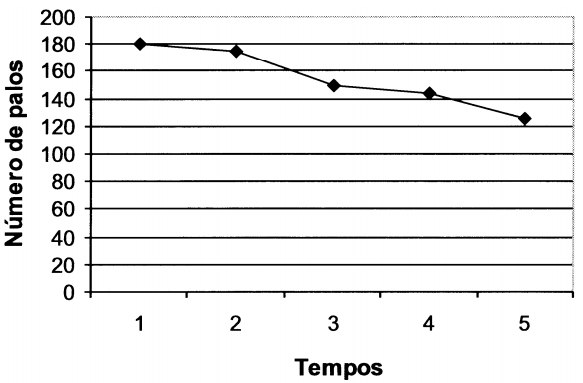
\includegraphics[width=0.76\textwidth]{./fig/grafico-rendimento/decrescente}
 \caption{Rendimento descendente ou decrescente.}
  Fonte: \cite{psicohood2018}.
 \label{fig:ascende}
\end{figure}


\textbf{Convexo ou parabólico} (NOR acima de 6): há um aumento da produção no 2º tempo, mantendo-se ou aumentando no 3º tempo, mas não continua com a disposição até o final da tarefa, voltando aproximadamente ao nível de produção inicial. Expressa ímpeto para iniciar as tarefas, que não se mantém até o final, podendo
estar relacionado a falta de planejamento das suas ações e do tempo. Se ocorrer em conjunto com alinhamento (direção das linhas) convexo, descendente ou em leque, pode indicar possíveis tendências depressivas.
É característico de pessoas que não concluem o que começam.

Ex.:
\begin{table*}[h]
\centering
\caption{Rendimento convexo ou parabólico \cite{psicohood2018} }
\label{tab:convexo} 

\begin{tabular}{|l|c|c|c|c|c|c|}
\hline Tempos       & 1     & 2     & 3    &  4     & 5     & Total \\ 
\hline Nº de traços & 116 & 130 & 141 & 137 & 115 & 639 \\ 
\hline    \multicolumn{2}{|l|}{ Diferenças}& 14   & 11    &4     & 22    & 51\\ 
\hline NOR = 7,9\\
\cline{1-11}
\end{tabular} 

\end{table*}

\begin{figure}[H]
 \centering
 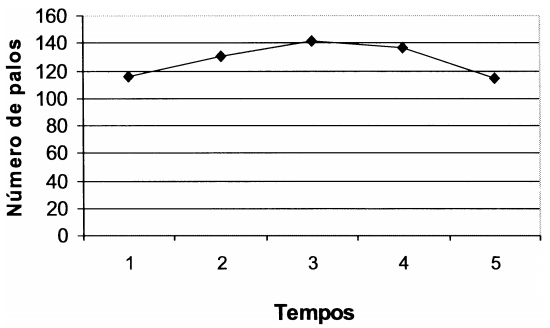
\includegraphics[width=0.76\textwidth]{./fig/grafico-rendimento/convexo}
 \caption{Rendimento convexo ou parabólico.}
  Fonte: \cite{psicohood2018}.
 \label{fig:convexo}
\end{figure}

\textbf{Côncavo} (NOR acima de 6): produção inicial mais alta, que diminui por uma falta de disposição durante a atividade
e recupera com a continuação da tarefa.

Ex.:
\begin{table}[h]
\centering
\caption{Rendimento côncavo\cite{psicohood2018} }
\label{tab:côncavo} 
\begin{tabular}{|l|c|c|c|c|c|c|}
\hline Tempos       & 1     & 2     & 3    &  4     & 5     & Total \\ 
\hline Nº de traços & 150 & 135 & 124 & 140 & 153 & 700 \\ 
\hline    \multicolumn{2}{|l|}{ Diferenças}& 15   & 11    &16     & 13    & 55\\ 
\hline NOR = 7,8\\
\cline{1-11}
\end{tabular} 

\end{table}

\begin{figure}[H]
 \centering
 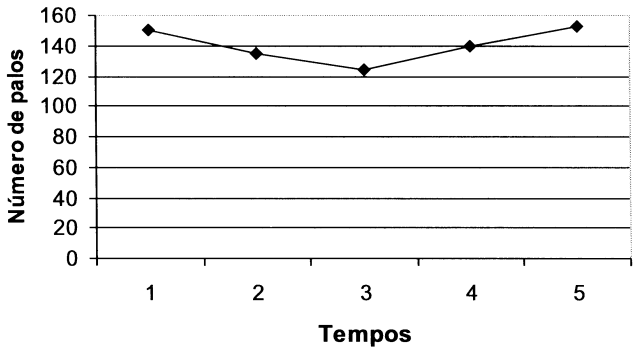
\includegraphics[width=0.76\textwidth]{./fig/grafico-rendimento/concavo}
 \caption{Rendimento côncavo.}
  Fonte: \cite{psicohood2018}.
 \label{fig:concavo}
\end{figure}

\textbf{Irregular ou oscilante }(NOR acima de 6): irregularidade no ritmo de trabalho, pode indicar estresse, falta de ânimo e disposição, motivação deficiente, ou interferência do estado emocional. Indica geralmente uma perturbação psíquica voluntária ou involuntária na administração do esforço.

Ex.:
\begin{table*}[h]
\centering
\caption{Rendimento irregular\cite{psicohood2018} }
\label{tab:irregular} 

\begin{tabular}{|l|c|c|c|c|c|c|}
\hline Tempos       & 1     & 2     & 3    &  4     & 5     & Total \\ 
\hline Nº de traços & 110 & 145 & 120 & 115 & 152 & 642 \\ 
\hline    \multicolumn{2}{|l|}{ Diferenças}& 35   & 25    &5     & 37    & 102\\ 
\hline NOR = 15,9\\
\cline{1-11}
\end{tabular} 

\end{table*}

\begin{figure}[H]
 \centering
 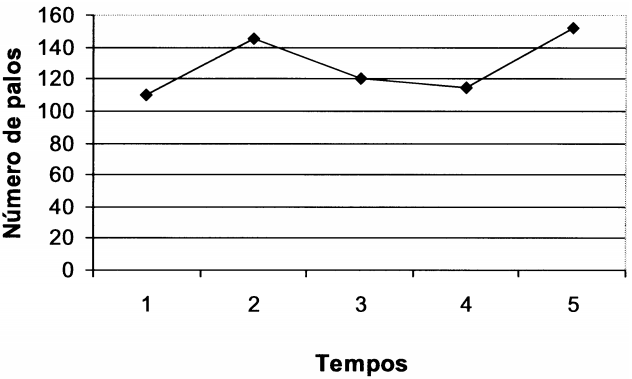
\includegraphics[width=0.76\textwidth]{./fig/grafico-rendimento/irregular}
 \caption{Rendimento irregular.}
  Fonte: \cite{psicohood2018}.
 \label{fig:irregular}
\end{figure}



\section{Visão computacional}
\label{sec:vc}
Visão computacional objetiva fazer com que os sistemas computacionais consigam enxergar, por meio da reprodução dos processos da visão humana utilizando software e hardware. Fazendo-se que o computador consiga realizar tarefas mais complexas e úteis na vida cotidiana e nos negócios como identificar doenças em raio-x, reconhecimento facial, ler sinais de trânsito, reconhecer pedestres, etc. \cite{dsAcademy2017}

Visão computacional é a combinação de várias técnicas de processamento de imagens  com o objetivo de identificar padrões, e reconhecer objetos em imagens. Ainda que a visão computacional já esteja sendo utilizada em diversas áreas de negócio, como no monitoramento de trânsito, identificar produtos e onde comprá-los, detecção de fraudes, reconhecimento de caracteres, monitoramento de fluxo de pessoas, identificação de pessoas entre outros. Ainda é uma tarefa muito complexa e está em evolução \cite{dsAcademy2017}.


Ensinar computadores a ver como os seres humanos é uma missão bem complexa, porque ainda não compreendemos por completo como o processo de visão realmente funciona \cite{dsAcademy2017}.

Conforme [Telles 2013 apud YANG 2007] é muito difícil criar sistemas de visão computacional que se assemelham  às  habilidades cognitivas dos  humanos, dentre as dificuldades estão a variação de iluminação, a dificuldade de generalizar objetos a partir de um conjunto pre-definido de imagens e as variações de posição do objeto em relação à câmera.

Diversos algorítimos foram desenvolvidos para extrair informações de imagens com a finalidade de automatizar tarefas na qual geralmente seriam feitas utilizando se da visão humana. Na visão humana  sabemos,  que  nossos olhos capturam as imagens e depois nosso cérebro realiza a análise e identificação do seu conteúdo. Na visão computacional realizamos uma série de etapas para reproduzir o processo da visão humana.

Dependendo do problema, todas as etapas explicadas a seguir são aplicadas, porém, isso não é uma regra, pode haver situações em que apenas algumas etapas já conseguem resolver o problema em questão utilizando-se de metologias diferentes  da apresentada.

Segundo \cite{digitalImgProcess2010} existem algumas etapas básicas na análise de dados em imagens que se dividem em: aquisição da imagem, pré-processamento, segmentação, descrição, reconhecimento e interpretação. Estas etapas estão englobadas em três áreas básicas: primeira, processamento de baixo nível, com funções que podem ser vistas como reações que não requerem comportamento inteligente; segunda processamento de nível intermediário, com extração e caracterização de componentes; e terceira processamento de alto nível, que utiliza-se de reconhecimento e interpretação. Na Figura \ref{fig:imgpdi} pode se ver todo esse processo.

\begin{figure}[H]
 \centering
 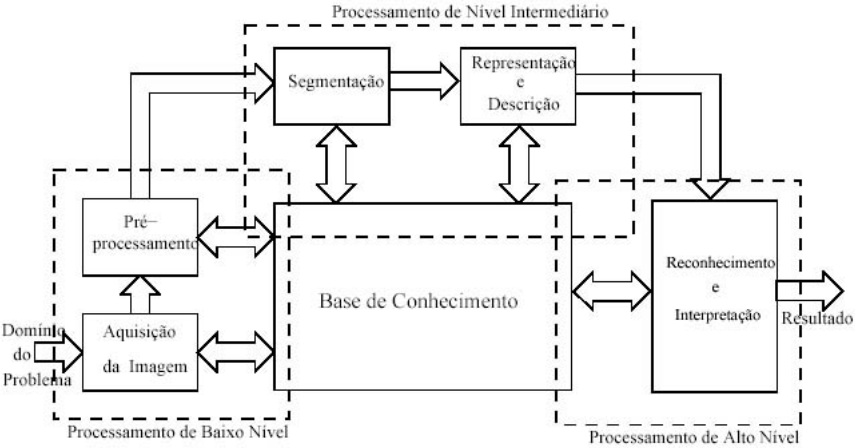
\includegraphics[width=0.89\textwidth]{./fig/fundamentacao/pdi2}
 \caption{Etapas de um sistema de visão computacional}
 \label{fig:imgpdi}
\end{figure}

Na etapa da aquisição da imagem acontece a captura e digitalização da imagem, por meio de um dispositivo de captura, nesse trabalho foi usado a câmera de um \textit{smartphone}. No pré-processamento, temos o tratamento da imagem, que pode ter vindo com ruídos e imperfeições intrínsecas da cena.  Na segmentação a imagem é dividida de acordo com as regiões de interesse, por exemplo os palos gravados na folha do teste. Na representação, são extraídas características relevantes ao domínio do problema e preparadas para o próximo passo. Na interpretação temos a atribuição de significado ao conjunto de objetos reconhecidos. 

\subsection{Aquisição de imagem}
\label{sub:aquis}

Existem diversos, dispositivos de captura de imagens, por exemplo, câmera, scanner, leitor biométrico, máquinas de raio-x, etc. A qualidade da imagem vai depender muito do dispositivo, e do ambiente onde esta sendo feito a aquisição, pois pode haver problemas, como falha mecânica do dispositivo, iluminação heterogênea, baixa resolução o que pode causar ruídos na imagem.

\subsection{Pré-processamento}
\label{sub:pre-process}

Nessa etapa, são aplicadas diversas operações tais como realce de contrastes, remoção de ruídos e suavização de regiões, melhorando a qualidade da mesma. Essas transformações são ditas de baixo nível, pois trabalham diretamente com os valores de intensidade de pixels, sem se importar nesse momento com informações relativas ao domínio do problema. O resultado é outra imagem de melhor qualidade que a original, isso aumenta as chances de sucesso dos processos seguintes [Filho & Neto, 1999].

Alguns exemplos de aplicação de filtros: a redução de ruídos, o controle do nível de brilho ou contraste, entre outras aplicações. 


\subsection{Segmentação}
\label{sub:segment}

Nesta etapa do pré-processamento a imagem é subdividida em partes de acordo com os objetos detectados na imagem. Cada uma dessas partes é uniforme e homogênea no tocante a algumas propriedades da imagem como textura e cor.

Os algoritmos de segmentação geralmente são baseados na busca pelas descontinuidades ou pelas similaridades dos níveis de cinza. \cite{digitalImgProcess2010} O objetivo da segmentação é agrupar um conjunto de pixels de mesma propriedade, para isso, não pode haver erro, pois isso pode comprometer o sucesso da análise da imagem.

Na descontinuidade, o particionamento da imagem é baseado no subconjunto de pontos de um objeto que o separa do restante da imagem, quer dizer, são representadas por alterações abruptas nos tons de cinza, cores e texturas. Na similaridade, a segmentação é baseada nos aspectos comuns dos pixels da imagem, inicialmente, o método começa com um pixel, e a partir deste pixel, examina-se seus vizinhos, numa determinada sequência, para decidir se eles possuem níveis de cinza similares, segundo o critério de similaridade escolhido, existem diversas técnicas de segmentação por similaridade,  uma delas é a limiarização a qual foi utilizada nesse trabalho.


\subsection{Representação e descrição}
\label{sub:rep-desc}

Após a etapa de segmentação é obtido um agregado de pixels segmentados. Pode ser necessário transformar os dados para uma forma adequada para o futuro processamento por computador. Neste caso podem ser utilizadas as representações por características externas (sua fronteira) ou características internas (os pixels que constituem a região). A representação por fronteira é adequada quando o foco está em características externas da forma,  por exemplo, em cantos. Uma representação por região é apropriada quando o foco está em propriedades internas do objeto como forma, cor ou textura. Dependendo do projeto é necessário usar às duas categorias de representação. Escolher a representação é apenas parte da solução para a transformação de dados brutos em uma forma conveniente para o processamento na próxima etapa. Um método para descrever os dados deve ser especificado, de maneira que as características de interesse sejam enfatizadas. Descrição, é utilizada na extração de atributos que tem como resultado, informação quantitativa ou que possa ser utilizada para diferenciar classes de objetos \cite{digitalImgProcess2010}.

Estes descritores devem ser representados por uma estrutura de dados adequada ao algoritmo de reconhecimento. Nessa etapa a entrada ainda é uma imagem, mas a saída é uma lista de dados correspondentes a imagem. Por exemplo, os descritores utilizados nesse trabalho para os descrever os palos foram as coordenadas x e y sua área, altura, largura e sua forma retangular. Neste caso, um vetor armazena essas características em seguida cada vetor é adicionado em um lista de dados. 

\subsection{Reconhecimento e interpretação}
\label{sub:rec-intr}

O reconhecimento faz a atribuição de rótulo a um objeto (por exemplo, “veículo”), tendo como base as informações fornecidas na etapa anterior pelo descritor e a interpretação atribui um significado a um conjunto de objetos reconhecidos. No exemplo de reconhecimento de caracteres, este passo seria responsável por identificar que um determinado conjunto de objetos, por exemplo, cinco números seguidos por um hífen e outros três números representa um CEP. O reconhecimento sobre o domínio do problema está codificado em sistema de processamento de imagens na forma de uma base de conhecimento. Este pode ser simples quanto o detalhamento de regiões de uma imagem na qual se sabe que a informação de interesse pode ser localizada, ou complexa, por exemplo, uma lista inter-relacionada de todos os principais defeitos possíveis em um problema de inspeção de materiais, isso vai depender do domínio do problema.\cite{digitalImgProcess2010}


\section{Imagem Digital}
\label{sec:img}

Uma imagem digital é representada por um matriz de linhas e colunas que definem cada ponto(x,y) na imagem. Cada ponto na matriz bidimensional é denominado pixel. Os pontos são coordenadas espaciais onde as linhas y e colunas x são definidos por um função bidimensional f(x,y), que corresponde ao valor do elemento e a intensidade do nível de cinza ou cor naquele ponto da matriz. Quando (x, y) e os valores de intensidade f são quantidades finitas e discretas, temos a imagem digital. \cite{ImgDigital2001} 

Na figura \ref{fig:imgDigital} temos uma imagem monocromática identificando sua origem  (0,0) e a posição dos eixos no plano cartesiano.

\begin{figure}[H]
 \centering
 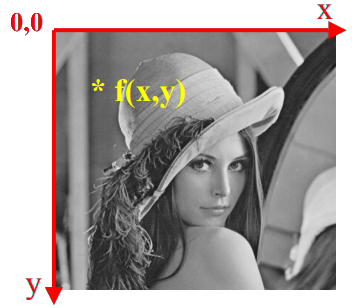
\includegraphics[width=0.60\textwidth]{./fig/fundamentacao/lenna}
 \caption{Demostração de uma Imagem digital}
  Fonte: \cite{imagemDigital2019}.
 \label{fig:imgDigital}
\end{figure}


\subsection{Sistemas de cores}
\label{sub:siscores}

\subsubsection{Escala de cinza}
\label{subsub:siscores-cinza}

A luz quando sem cor é chamada monocromática. A intensidade da luz monocromática pode variar entre o preto (0) , passando por tons de cinza, até o branco (255), chamado de nível de cinza. Essa variação na intensidade é conhecida por escala de cinza. 
Essa escala de cinza possui uma variação de 256 tonalidades, pois possuem 8 bits para representarem essas tonalidades. 

Para diminuir o peso do processamento da imagem, antes de qualquer operação, as imagens devem ser convertidas para escala de cinza.\cite{digitalImgProcess2010}


\subsubsection{Sistema de cores RGB}
\label{subsub:siscores-RGB}

O padrão de cores RGB trabalha com as cores   vermelho (\textit{Red}), verde (\textit{Green}) e  azul(\textit{Blue}). Cada uma dessas cores possui uma variação de 256 valores.  Cada cor pode receber um valor de intensidade de 0 até 255, e podem ser combinadas gerando mais de 16,7 milhões de cores distintas.  A Figura  \ref{fig:imgCORES} mostra um exemplo de combinações das cores RGB.  Neste trabalho foi utilizado a biblioteca Opencv que trabalha com a imagem no padrão BGR, a diferença é somente a ordem das cores.

\begin{figure}[H]
 \centering
 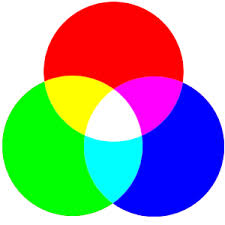
\includegraphics[width=0.30\textwidth]{./fig/fundamentacao/cores-rgb}
 \caption{cores RGB}
 Fonte: \cite{coresRGB}.
 \label{fig:imgCORES}
\end{figure}

\subsubsection{Sistema de cores HSV}
\label{subsub:siscores-HSV}


HSV é abreviatura para os componentes de tom (\textit{hue}), saturação (\textit{saturation}) e valor (\textit{value}). Este sistema é conhecido também como HSB (\textit{hue, saturation, brightness}). 
\textit{Hue} :  é o tipo de cor ou tonalidade, pode ser vermelho, amarelo, azul, etc. Pode ter valores entre 0 e 360, mas para algumas aplicações, este valor é normalizado de 0 a 100\%.
\textit{Saturation} : determina a profundidade ou pureza da cor (de esmaecida a intensa) Pode ter valores entre 0 e 100\% sendo mais saturada aquela mais próxima ao 100\%.
\textit{Value}: determina a intensidade percebida ( cor mais clara ou mais escura)
na Figura \ref{fig:imgHSV} é mostrado a representação desse sistema.

\begin{figure}[H]
 \centering
 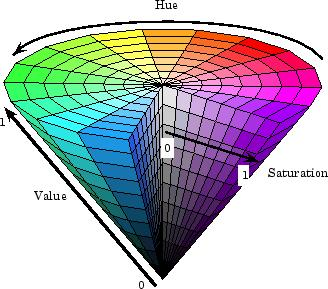
\includegraphics[width=0.30\textwidth]{./fig/fundamentacao/hsvcone}
 \caption{cores HSV}
 Fonte: \cite{coresHSV}
 \label{fig:imgHSV}
\end{figure}

\section{Histograma}
\label{sec:histograma}

No processamento de imagem o histograma calcula quantos pixels existem naquela tonalidade. Estes valores são geralmente representados por um gráfico de barras no qual cada retângulo representa um intervalo e sua altura representa a frequência naquele intervalo través do histograma.
Com a imagem em escala de cinza o histograma representa a distribuição dos níveis de cinza da imagem. O histograma possibilita um melhor entendimento da qualidade da imagem como nível de contraste e seu brilho. \cite{ImgDigital2001}

Na Figura \ref{subfig:histograma} tem a representação dos histogramas de quatro imagens básicas.
\begin{figure}[h]
 \centering
  \subfigure[][Imagem escura.]
   {
    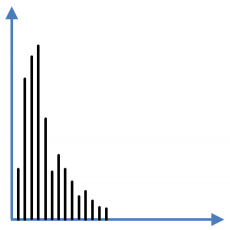
\includegraphics[width=0.22\textwidth]{./fig/fundamentacao/a}
    \label{subfig:hist-a}
   } \qquad
    \subfigure[][Imagem clara.]
   {
    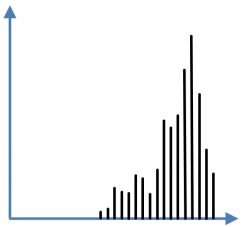
\includegraphics[width=0.22\textwidth]{./fig/fundamentacao/b}
    \label{subfig:hist-b}
   } \qquad
   \subfigure[][Imagem de baixo contraste.]
   {
    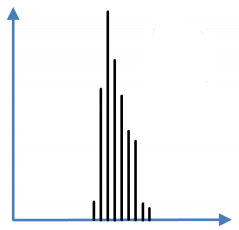
\includegraphics[width=0.22\textwidth]{./fig/fundamentacao/c}
    \label{subfig:hist-c}
   } \qquad
  \subfigure[Imagem de alto contraste.]
   {
    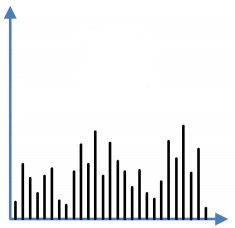
\includegraphics[width=0.22\textwidth]{./fig/fundamentacao/d}
    \label{subfig:hist-d}
   }
   \caption{{\subref{subfig:hist-a}} , {\subref{subfig:hist-b}}, {\subref{subfig:hist-c}} e {\subref{subfig:hist-d}} Histogramas referentes a quatro tipos básicos de imagens \cite{digitalImgProcess2010} }
  \label{subfig:histograma}
\end{figure}


\subsection{Equalização do Histograma}
\label{sub:equa-hist}

A equalização do histograma procura redistribuir os valores dos níveis de cinza na imagem, para se obter um histograma uniforme, no qual o número de pixels de qualquer nível é praticamente o mesmo, isso melhora o contraste da imagem.
É utilizado para corrigir problemas de contraste na imagem monocromática, causados por iluminação deficiente, excessiva ou mesmo de calibração incorreta do obturador. Essa técnica também podem ser aplicada a partes da imagem, em janelas m x n, para realçar detalhes minuciosos de pequenas porções da imagem \cite{pdi99}.

A Figura \ref{subfig:equl-histograma} apresenta um exemplo de aplicação da técnica de equalização de histograma
para aumentar o contraste de uma imagem 446 x 297 com 256 tons de cinza \cite{pdi99}.

\begin{figure}[h]
 \centering
  \subfigure[][Imagem original.]
   {
    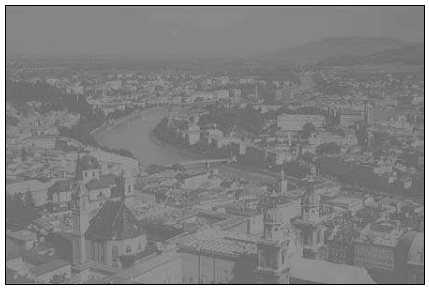
\includegraphics[width=0.30\textwidth]{./fig/fundamentacao/hist-a}
    \label{subfig:histi-a}
   } \qquad
    \subfigure[][Histograma da imagem original.]
   {
    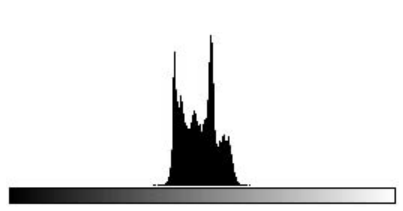
\includegraphics[width=0.30\textwidth]{./fig/fundamentacao/hist-grafico-b}
    \label{subfig:hist-grafico-b}
   } \qquad
   \subfigure[][Imagem equalizada.]
   {
    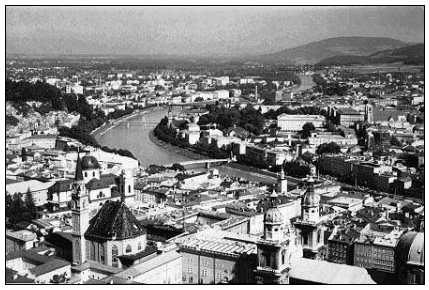
\includegraphics[width=0.30\textwidth]{./fig/fundamentacao/hist-equl-c}
    \label{subfig:histi-c}
   } \qquad
  \subfigure[Histograma da imagem equalizada.]
   {
    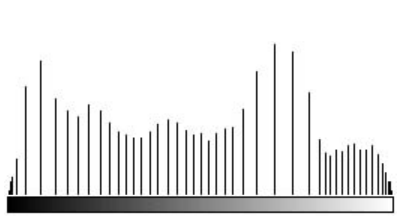
\includegraphics[width=0.30\textwidth]{./fig/fundamentacao/hist-grafico-d}
    \label{subfig:hist-grafico-d}
   }
   \caption{ Aplicação da equalização de histograma a imagens com baixo contraste \cite{pdi99}}
  \label{subfig:equl-histograma}
\end{figure}



\section{Limiarização }
\label{sec:limiar}

O limiarização (\textit{Thresholding}) tem como objetivo dividir uma imagem em regiões separando fundo e o objeto, tendo como base a análise de níveis de cinza em relação a um limiar T. Esse processo transforma uma imagem de escala de cinza para uma com pixels pretos e brancos, essa transformação consiste em comparar cada pixel da imagem com o valor do limiar T, qualquer ponto (x,y) na imagem em que f(x,y) > T esse ponto recebera o valor \textbf{1} identificando como sendo do objeto e caso contrário, o ponto receberá o valor \textbf{0} este será o fundo (background) da imagem, tendo como saída uma imagem binária g(x,y) \cite{digitalImgProcess2010}.

\begin{center}
    $g(x,y)= \left\{\begin{matrix}
        & 1 \ se \  \textit{f}(x,y) > T   \\ 
        & 0 \ se \  \textit{f}(x,y) \leq  T
    \end{matrix}\right\\$ 
\end{center} 

Por convenção são utilizados os valores de intensidade 0 e 1, mas podem ser utilizados dois valores quaisquer, desde que sejam distintos. A definição de um bom limiar é essencial para o que processo de limiarização seja satisfatório. Devido às variações de brilho e contraste, a definição de um limiar não é simples. 

Existem diversas variantes de limiarização a mais simples define o seu limiar único T baseado na análise do histograma da imagem. Na Figura \ref{subfig:limiarizacao} pode se ver um exemplo de definição de limiar baseado no histograma, na imagem temos dois picos e um vale um caso de limiarização mais simples \cite{pdi99}.

\begin{figure}[h]
 \centering
   \subfigure[][Histograma original.]
   {
    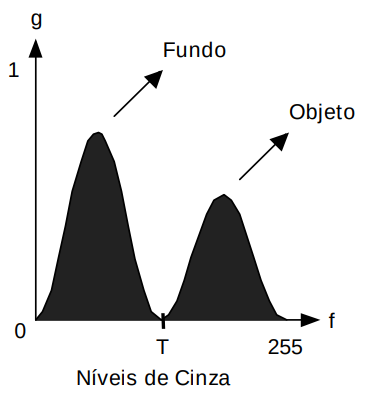
\includegraphics[width=0.22\textwidth]{./fig/fundamentacao/hist-cinza}
    \label{subfig:hist-cinza}
   } \qquad
  \subfigure[Histograma da imagem binarizada.]
   {
    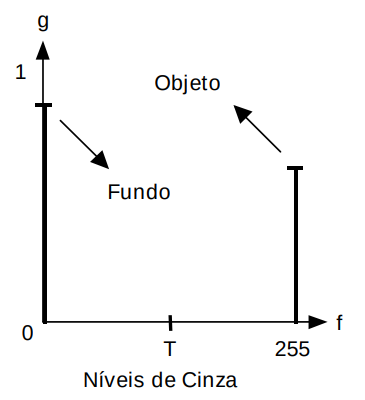
\includegraphics[width=0.22\textwidth]{./fig/fundamentacao/hist-bin}
    \label{subfig:hist-bin}
   }
   \caption{ Limiarização de uma imagem monocromática utilizando limiar T. \cite{pdi99}}
  \label{subfig:limiarizacao}
\end{figure}

Quando o limiar T é aplicado na imagem inteira temos a limiarização global e quando esse limiar T depende de propriedades de pixels de uma vizinhança ou de coordenadas espaciais(x,y) temos a limiarização adaptativa ou dinâmica.\cite{digitalImgProcess2010}

A limiarização é muito importante para o sucesso na segmentação de objetos na imagem.

\section{Filtro espacial de suavização (\textit{blur})}
\label{sec:blur}

O filtro de suavização ou borramento, tem a função de embaçamento na imagem, diminuindo a definição, contribuindo para a redução de ruídos. Esse filtro normalmente é usado no pré-processamento para a segmentação de objeto e conexão de pequenas descontinuidades em linhas ou curvas.\cite{digitalImgProcess2010}

A suavização é obtida pela média dos pixels vizinhos tendo como base uma máscara. Esse filtro de suavização também é conhecido como filtro passa baixa. A suavização elimina mudanças bruscas na intensidade entre os pixels, causando perca de nitidez reduzindo assim os ruídos, porém deve-se ter cuidado, pois isso pode prejudicar a detecção de bordas.

Na figura \ref{subfig:suavizacao}, é apresentado a aplicação de suavização de uma imagem.

\begin{figure}[h]
 \centering
   \subfigure[][Imagem original.]
   {
    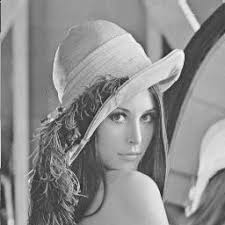
\includegraphics[width=0.26\textwidth]{./fig/fundamentacao/lenna-gray}
    \label{subfig:blur-original}
   } \qquad
   \subfigure[][Imagem suavizada com máscara 3x3.]
   {
    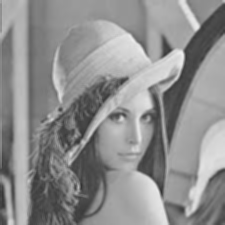
\includegraphics[width=0.26\textwidth]{./fig/fundamentacao/lenna-blur-3}
    \label{subfig:blur-3}
   } \qquad
  \subfigure[Imagem suavizada com máscara 5x5.]
   {
    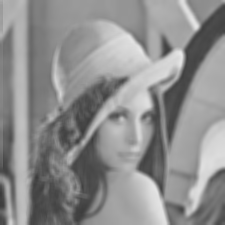
\includegraphics[width=0.26\textwidth]{./fig/fundamentacao/lenna-blur-5}
    \label{subfig:blur-5}
   }
   \caption{ Aplicação do filtro da média com mascara 3x3 e 5x5.}
      Fonte: \cite{imagemDigital2019}
  \label{subfig:suavizacao}
\end{figure}

\section{Detecção de bordas}
\label{sec:bordas}

Bordas(\textit{\textbf{edges}}) podem ser definidas como o limite entre duas regiões cujos níveis de cinza sofrem uma mudança bruta de brilho na imagem. As bordas são os contornos dos objetos, e são muito importantes para identificar e segmentar objetos em imagens.\cite{digitalImgProcess2010}

As bordas são utilizadas com mais frequência do que detecção de pontos e linhas, apesar de que pontos e linhas isolados também são utilizados em segmentação, porém,  não são muito frequentes em aplicações práticas. \cite{digitalImgProcess2010}

O reconhecimento de bordas não é trivial, devido a problemas como variação na iluminação, um objeto atrás do outro que geralmente será mais escuro; um objeto perpendicular à iluminação é mais claro que um que esteja paralelo; mudanças das propriedades de material, textura e cor; características como reflexão e refração tudo isso é um grande desafio na detecção de bordas. 

Existem diversas técnicas para detecção de borda uma delas é a utilização  de operadores diferenciais com uso de máscaras de convolução. Esses operadores encontram as variações nos níveis de pixels com a aplicação das derivadas primeira e segunda. Consegue-se detectar as bordas fazendo a convolução da máscara  para cada pixel na imagem.\cite{digitalImgProcess2010}

Neste trabalho foram testados dois operadores o Canny e o Sobel sendo o Sobel o que apresentou um melhor resultado.
O Sobel utiliza o gradiente para a determinação da borda na imagem. A Figura \ref{subfig:mascara-sobel} ilustra as máscaras utilizadas pelo operador Sobel na detecção de bordas horizontais e verticais.

\begin{figure}[h]
 \centering
   \subfigure[][Máscara horizontal.]
   {
    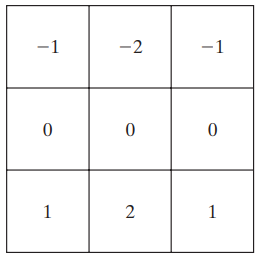
\includegraphics[width=0.20\textwidth]{./fig/fundamentacao/m-sobel-h}
    \label{subfig:blur-original}
   } \qquad
   \subfigure[][Máscara Vertical.]
   {
    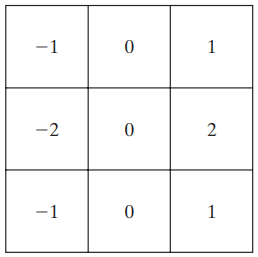
\includegraphics[width=0.20\textwidth]{./fig/fundamentacao/m-sobel-v}
    \label{subfig:blur-3}
   } \qquad
  \subfigure[Máscara de posição.]
   {
    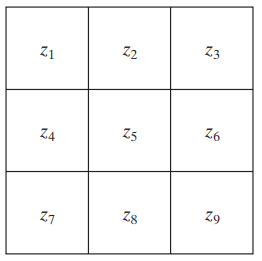
\includegraphics[width=0.20\textwidth]{./fig/fundamentacao/m-sobel-z}
    \label{subfig:blur-5}
   }
   \caption{ Máscaras utilizadas no operador Sobel. \cite{digitalImgProcess2010}}
  \label{subfig:mascara-sobel}
\end{figure}

As derivadas aplicadas nas máscaras do operador de Sobel são mostradas nas equações (1) e (2). Por meio delas consegue-se estimar a presença de mudança de região  de tons claros e escuros.

\ (1) 
\begin{center}
    $g(x)=\frac{\partial f(x,y)}{\partial x}=(Z_{7}+2Z_{8}+Z_{9})-(Z_{1}+2Z_{2}+Z_{3})$ 
\end{center}

\ (2)
\begin{center}
    $g(y)=\frac{\partial f(x,y)}{\partial y}=(Z_{3}+2Z_{6}+Z_{9})-(Z_{1}+2Z_{4}+Z_{7})$ 
\end{center}

Para cada ponto da imagem  é calculada na equação (3) a aproximação do gradiente combinando o resultado (1) e (2).

\ (3)
\begin{center}
    $G=\sqrt{g(x)^{2} + g(y)^{2}}$
\end{center}

O resultado do deslocamento das máscaras para todos os pixel é uma de gradiente com as mesmas dimensões da original. \cite{digitalImgProcess2010}

Na figura \ref{subfig:filtro-sobel} vemos a aplicação do filtro Sobel.

\begin{figure}[h]
 \centering
   \subfigure[][Imagem original.]
   {
    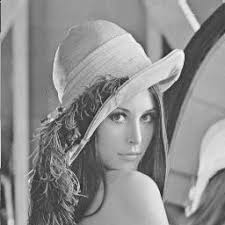
\includegraphics[width=0.25\textwidth]{./fig/fundamentacao/lenna-gray}
    \label{subfig:sobel-original}
   } 
   \qquad
  \subfigure[Imagem com filtro de Sobel.]
   {
    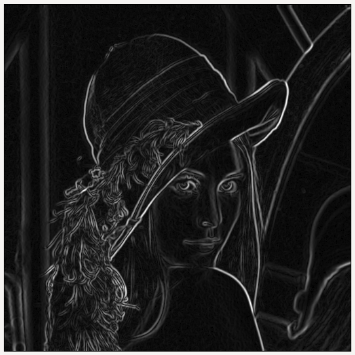
\includegraphics[width=0.25\textwidth]{./fig/fundamentacao/lenna-sobel}
    \label{subfig:sobel-filtro}
   }
   \caption{ Aplicação do filtro de Sobel para detectar bordas.}
  \label{subfig:filtro-sobel}
\end{figure}

\section{Morfologia Matemática}
\label{sec:morfologia}
A morfologia matemática tem em sua essência extrair informações relativas à geometria e à topologia de uma imagem, realizando transformações por um elemento estruturante. Algumas das aplicações dessa técnica no processamento de imagens são:  realce, filtragem, segmentação, detecção de bordas, esqueletização e afinamento de imagens. \cite{pdi99} Neste trabalho foram utilizadas duas operações fundamentais da morfologia matemática a dilatação e a erosão.

Na erosão os pixels que formam um determinado padrão são retirados da imagem, e na dilatação é ao contrário os pixels são adicionados à imagem de acordo com a forma do elemento estruturante escolhido.\cite{digitalImgProcess2010}

A técnica de operações morfológicas é baseada na teoria dos conjuntos, na qual os conjuntos representam a forma dos objetos em uma imagem. Em imagens binárias os conjuntos de pixels pertencem ao espaço bidimencional inteiro $Z^{2}$ e cada elemento do conjunto é um vetor 2-D, cujas coordenadas (x,y) representam os pixels pretos (por convenção) na imagem.\cite{pdi99}

\subsection{Dilatação}
\label{subsec:morfologia-dila}

Sejam A e B conjuntos no espaço $Z^{2}$ o processo de dilatação se baseia na reflexão\footnote{ Na reflexão, todos os elementos de B em torno da origem desse conjunto são refletidos. Representada por $\hat{B}$ é simplesmente o conjunto dos pontos em B cujas coordenadas (x,y) foram substituídas por (-x,-y) }  de B em torno de sua origem e depois deslocar esta reflexão de x. A dilatação de A por B é, então, o conjunto de todos os x deslocamentos para os quais a interseção de $(\hat{B})_{x}$ e A influi pelo menos um elemento diferente de zero. Com base nesta interpretação, temos a seguinte equação, sendo B o elemento estruturante (ES).\cite{pdi99}

\begin{center}
    $A \oplus B = \begin{Bmatrix}
    x\mid \left [ (\hat{B})_{x}\cap A \right  ] \subseteq A 
    \end{Bmatrix}$
\end{center}

A dilação diferentemente da erosão provoca o engrossamento dos objetos na imagem, de acordo com o elemento estruturante escolhido. Na figura \ref{subfig:dilatacao} temos um exemplo de dilatação, onde no centro temos o elemento estruturante que vai percorrer a imagem, e cada vez que seu pixel central coincidir com o mesmo pixel na imagem original, o elemento estruturante é inserido na imagem tendo como resultado uma imagem dilatada.

\begin{figure}[h]
 \centering
  \subfigure[Imagem original \textbf{A}]
   {
    
\includegraphics[width=0.20\textwidth]{./fig/fundamentacao/a-dilat}
     \label{subfig:a-dilat}
   }
   \qquad
  \subfigure[ES \textbf{B = $\hat{\textbf{B}}$}]
   {
    
\includegraphics[width=0.10\textwidth]{./fig/fundamentacao/e-dilat}
    \label{subfig:e-dilat}
   }
   \qquad
  \subfigure[Resultado da dilatação \textbf{A $\oplus$ B }]
   {
    
\includegraphics[width=0.25\textwidth]{./fig/fundamentacao/ab-dilat}
    \label{subfig:ab-dilat}
   }
   \caption{ Exemplo de dilatação. \cite{pdi99}}
  \label{subfig:dilatacao}
\end{figure}

\subsection{Erosão}
\label{subsec:morfologia-erosao}

A erosão provoca o afinamento do objeto na imagem binária, sendo que elementos menores que o elemento estruturante, incluindo pontos isolados, são removidos contribuindo para a remoção de ruídos. \cite{digitalImgProcess2010}

Sendo A e B como conjunto de $Z^{2}$, temos que a erosão de A por B indicada por A $\ominus$ B,  é o conjunto de todos os pontos x de forma que B, transladado \footnote{A translação na matemática é o movimento de um elemento de um ponto a outro. É análoga à operação de rotacionar } de x, está contido em A. Assim sendo A representa o objeto na imagem e B o elemento estruturante. Por B estar contido em A, o elemento estruturante não em comum com o fundo, sendo $A^{c}$ o complemento do conjunto A, ou seja, o fundo da imagem, então a erosão pode ser expressa com a seguinte equação:
\cite{pdi99}

\begin{center}
    $A \ominus  B = \begin{Bmatrix}
    x\mid   (B)_{x}\cap A^{c}    =  \varnothing 
    \end{Bmatrix} $
\end{center}

A diferença da erosão para a dilatação é que quando o pixel central do elemento estruturante coincide com o da imagem, ao invés de acrescentar os pixels desse elemento, esses são retirados da imagem. Então a imagem resultante será menor que a original sofrendo a erosão. Na Figura \ref{subfig:dilatacao} temos o exemplo de erosão.

\begin{figure}[h]
 \centering
  \subfigure[Imagem original \textbf{A}]
   {
    
\includegraphics[width=0.25\textwidth]{./fig/fundamentacao/a-dilat}
     \label{subfig:a-dilat}
   }
   \qquad
  \subfigure[ ES \textbf{ B = $\hat{\textbf{B}}$}]
   {
    
\includegraphics[width=0.10\textwidth]{./fig/fundamentacao/e-dilat}
    \label{subfig:e-dilat}
   }
   \qquad
  \subfigure[Resultado da erosão \textbf{A $\ominus$ B }]
   {
    
\includegraphics[width=0.25\textwidth]{./fig/fundamentacao/ab-erosao}
    \label{subfig:ab-dilat}
   }
   \caption{ Exemplo de erosão. \cite{pdi99}}
  \label{subfig:dilatacao}
\end{figure}